\documentclass[resume]{subfiles}


\begin{document}
\section{Modèles dynamiques}
\subsection{Rétroaction positive}

\begin{figure}[H]
    \centering
    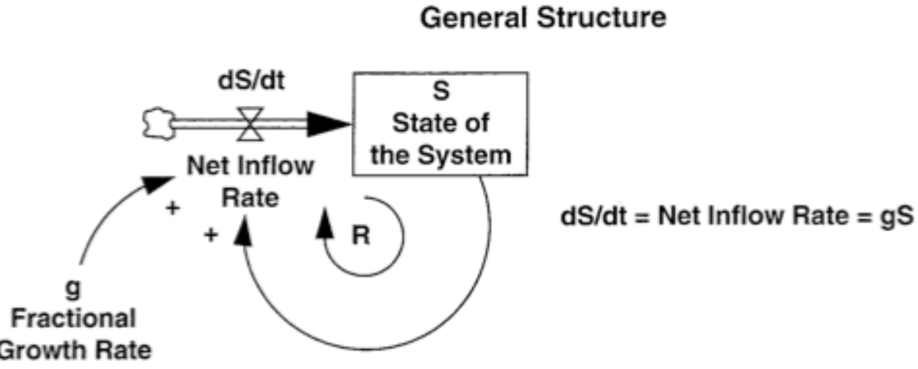
\includegraphics[width=1\columnwidth]{Figures/FDM_1.png}
\end{figure}

Le stock accumule du inflow $S(t)=S(0)e^{gt}$ 

Le temps de doublement du stock est de $2S(0)=S(0)e^{gt_d}$ on a donc $t_d=\frac{ln(2)}{g}=\frac{70}{100g}$

\subsection{Rétroaction négative et décroissance exponentielle}

\begin{figure}[H]
    \centering
    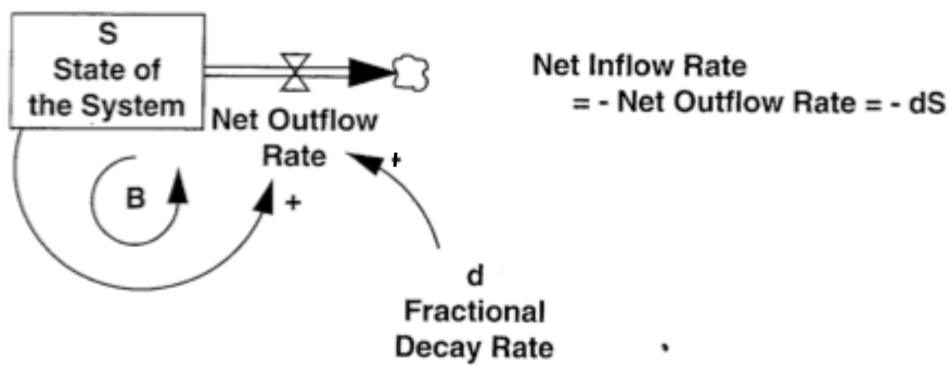
\includegraphics[width=1\columnwidth]{Figures/FDM_2.png}
\end{figure}

Le stock perd du outflow $S(t)=S(0)e^{-dt}$ 

Le temps de division par 2 du stock est de $t_d=ln(2)\tau=0.70\tau$ 

\subsection{Système non linéaires croissance en S}

\begin{figure}[H]
    \centering
    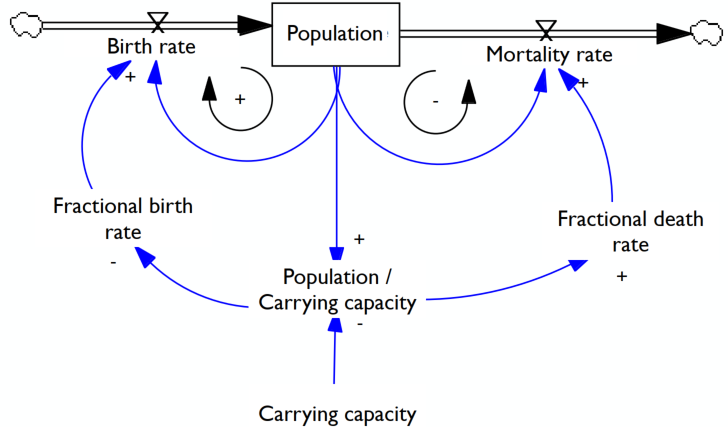
\includegraphics[width=1\columnwidth]{Figures/FDM_3.png}
\end{figure}

L'équation du système est $\frac{dP}{dt}=b(\frac{P}{C})P-d(\frac{P}{C})P$  

La croissance nette est une fonction de la population P : $\frac{dP}{dt}=g(P,C)P=g(1-\frac{P}{C})P$ 

Modèle logistique : $g(1-\frac{P}{C})$ 

Equation logistique : $P(t)= \frac{C}{1+[\frac{C}{P(0)}-1]e^{-gt}}$ 

\subsection{Modèle SI et SIR}
\begin{itemize}
\item S : susceptibles
\item I : infectés
\item R : rétablit
\end{itemize}

\begin{figure}[H]
    \centering
    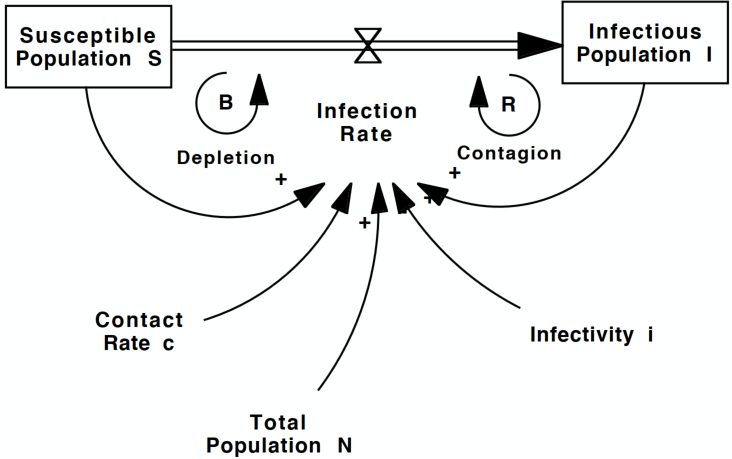
\includegraphics[width=1\columnwidth]{Figures/SI_1.png}
\end{figure}

\subsubsection{Equation du modèle SI}

$N=S+I \rightarrow \frac{dS}{dt}=-(ciS)\frac{I}{N}= -(I_R)$ IR = Infection Rate $\frac{dI}{dt}=ci\cdot I(1-\frac{I}{N})$ 

\begin{figure}[H]
    \centering
    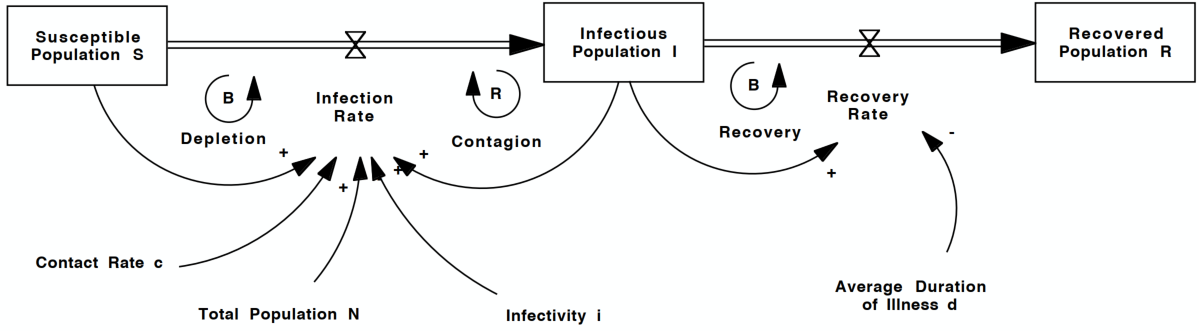
\includegraphics[width=1\columnwidth]{Figures/SIR_1.png}
\end{figure}

\subsubsection{Equation du modèle SIR}

\begin{align*}
\frac{dS}{dt}&=-(ciS)\frac{I}{N}\\
R_R&=\frac{I}{d}\\
\frac{dI}{dt} &= (ciS)\frac{I}{N}-\frac{I}{d}\\
\frac{dR}{dt} &= \frac{I}{d}\\
N&=S+I+R
\end{align*}


Point de bascule $I_R > R_R \rightarrow ciS(\frac{I}{N}) > \frac{I}{d}$ ou $cid(\frac{S}{N} > 1)$ 

\subsection{Retard}

Un retard est un processus dont la sortie correspond à l’entrée translatée dans le temps


\end{document}